% Ch1: overall thesis concept.
% Stage 1 adapts the VAE so the latent space can represent 4-channel CFD fields.
% Stage 2 trains the DiT in that latent space: from z_0 (the encoded initial
% condition) and gamma it generates z_1..z_13, which the decoder turns back
% into the physical trajectory. The encoded ground-truth z_1..z_13 are only the
% flow-matching target during training (dashed).
\documentclass[tikz,border=4pt]{standalone}
\usepackage{amsmath,amssymb}
\usetikzlibrary{arrows.meta,positioning,calc}
% Shared colours for the thesis TikZ figures. Same reference palette as
% scripts/thesis_figures.py (dataviz light mode), so diagrams and plots match.
\definecolor{ink}{HTML}{0B0B0B}
\definecolor{ink2}{HTML}{52514E}
\definecolor{muted}{HTML}{898781}
\definecolor{hair}{HTML}{C3C2B7}
\definecolor{neutralfill}{HTML}{F0EFEC}
\definecolor{blue}{HTML}{2A78D6}
\definecolor{bluefill}{HTML}{CDE2FB}
\definecolor{bluedark}{HTML}{184F95}
\definecolor{orange}{HTML}{EB6834}
\definecolor{orangefill}{HTML}{FBE0D3}
\definecolor{aqua}{HTML}{1BAF7A}
\definecolor{aquafill}{HTML}{D2F0E4}
\definecolor{violet}{HTML}{4A3AA7}
\definecolor{violetfill}{HTML}{E3E0F6}

% Trainable modules: orange fill + solid border. Frozen: neutral fill,
% dashed border, and every figure also labels the state in text.
\tikzset{
  every node/.style={font=\small, text=ink},
  box/.style={draw=hair, rounded corners=2pt, align=center, inner sep=4pt, line width=0.6pt},
  trainable/.style={box, fill=orangefill, draw=orange, line width=0.8pt},
  frozen/.style={box, fill=neutralfill, draw=muted, dashed},
  data/.style={box, fill=bluefill, draw=blue},
  latent/.style={box, fill=violetfill, draw=violet},
  cond/.style={box, fill=aquafill, draw=aqua},
  arr/.style={-{Stealth[length=5pt]}, draw=ink2, line width=0.7pt},
  note/.style={font=\footnotesize, text=ink2, align=center},
}


\newcommand{\framestack}[3]{% #1 name, #2 x, #3 y
  \foreach \k in {2,1,0} {
    \node[draw=blue, fill=bluefill, minimum width=1.0cm, minimum height=1.0cm, rounded corners=1pt, line width=0.6pt]
      (#1\k) at ($(#2,#3)+(\k*0.12,\k*0.12)$) {};
  }
}
% latent strip: first cell aqua (z_0), the rest violet; #4 = 1 draws the z_0 cell
\newcommand{\latentstrip}[4]{% #1 name, #2 x, #3 y
  \foreach \k in {0,...,6} {
    \ifnum\k=0
      \ifnum#4=1
        \node[draw=aqua, fill=aquafill, minimum width=0.26cm, minimum height=0.6cm, line width=0.5pt] (#1\k) at ($(#2,#3)+(\k*0.32,0)$) {};
      \else
        \node[draw=hair, fill=white, dashed, minimum width=0.26cm, minimum height=0.6cm, line width=0.5pt] (#1\k) at ($(#2,#3)+(\k*0.32,0)$) {};
      \fi
    \else
      \node[draw=violet, fill=violetfill, minimum width=0.26cm, minimum height=0.6cm, line width=0.5pt] (#1\k) at ($(#2,#3)+(\k*0.32,0)$) {};
    \fi
  }
}

\begin{document}
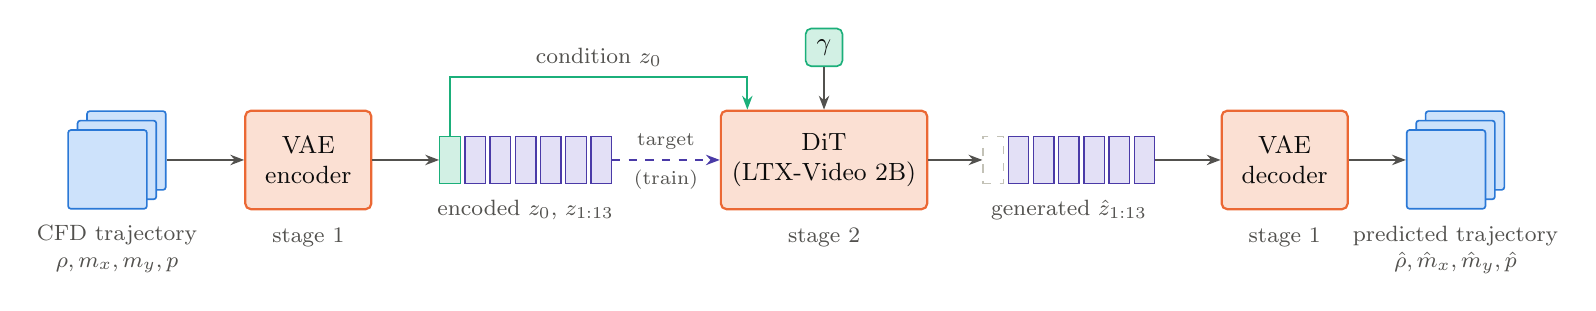
\begin{tikzpicture}
  \framestack{in}{0}{0}
  \node[note, anchor=north] at ($(in0.south)+(0.12,-0.08)$) {CFD trajectory\\$\rho, m_x, m_y, p$};

  \node[trainable, minimum height=1.25cm, minimum width=1.6cm] (enc) at (2.55,0.12) {VAE\\encoder};
  \latentstrip{lat}{4.35}{0.12}{1}
  \node[note, anchor=north] at ($(lat3.south)+(0,-0.08)$) {encoded $z_0$, $z_{1:13}$};

  \node[trainable, minimum height=1.25cm, minimum width=2.2cm] (dit) at (9.1,0.12) {DiT\\(LTX-Video 2B)};
  \node[cond] (gam) at (9.1,1.55) {$\gamma$};

  \latentstrip{pred}{11.25}{0.12}{0}
  \node[note, anchor=north] at ($(pred3.south)+(0,-0.08)$) {generated $\hat z_{1:13}$};

  \node[trainable, minimum height=1.25cm, minimum width=1.6cm] (dec) at (14.95,0.12) {VAE\\decoder};
  \framestack{out}{17.0}{0}
  \node[note, anchor=north] at ($(out0.south)+(0.12,-0.08)$) {predicted trajectory\\$\hat\rho, \hat m_x, \hat m_y, \hat p$};

  \draw[arr] (in2.east |- enc) -- (enc.west);
  \draw[arr] (enc.east) -- (lat0.west);
  \draw[arr] (gam) -- (dit);
  \draw[arr, draw=aqua] (lat0.north) -- ++(0,0.75) -| node[pos=0.25, above, note] {condition $z_0$} ($(dit.north west)+(0.35,0)$);
  \draw[arr, dashed, draw=violet] (lat6.east) -- node[above, note, font=\scriptsize] {target} node[below, note, font=\scriptsize] {(train)} (dit.west);
  \draw[arr] (dit.east) -- (pred0.west);
  \draw[arr] (pred6.east) -- (dec.west);
  \draw[arr] (dec.east) -- (out0.west |- dec);

  % which stage trains which module
  \node[note, anchor=north] at ($(enc.south)+(0,-0.1)$) {stage 1};
  \node[note, anchor=north] at ($(dit.south)+(0,-0.1)$) {stage 2};
  \node[note, anchor=north] at ($(dec.south)+(0,-0.1)$) {stage 1};
\end{tikzpicture}
\end{document}
